\section{Data and Simulator Choices}\label{sec:data-and-simulator-choices}
\paragraph In this section, we discuss the data and simulator choices for our experiments.

\subsection{Gym-Graph-Traffic}\label{subsec:gym-graph-traffic}
\paragraph Gym-graph-traffic is an OpenAI Gym-compatible road traffic simulator that provides a platform for studying and experimenting with various traffic scenarios. To use the simulator, users can easily install it from the provided GitHub repository\footnote{https://github.com/rltraffic/gym-graph-traffic} and run examples using Python scripts like \emph{minimal.py}. The simulator's configuration is customizable through parameters available in the \emph{params.py} file, allowing users to adjust aspects such as episode duration, step length, and possible actions per intersection.
\begin{figure}[H]
    \centering
    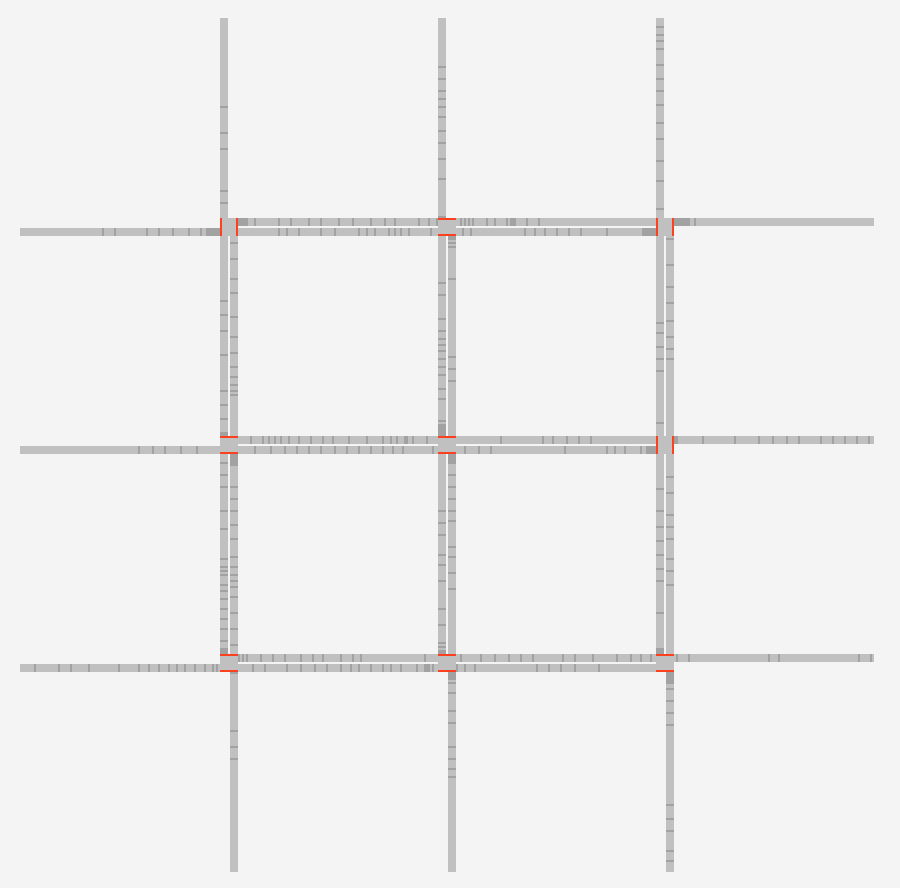
\includegraphics[width=10cm]{assets/gym-traffic}
    \caption{Gym-graph-traffic Simulator}
    \label{fig:gym-traffic}
    \small
    General interface of Gym-graph-traffic that allows us to simulate urban environment with a lot of entities
\end{figure}
The simulator operates on different time units, such as Experiment, Episode, Step, and Update, each representing specific durations in real-time seconds. Actions in the simulator are represented as integers and can be translated to a base x representation. By providing observation vectors for the average number of cars and average speed per road segment, users can monitor and evaluate traffic performance. With the option to choose from several preset road network configurations, the simulator offers flexibility in studying various traffic environments. Although not yet supporting Gym-like rendering, rendering options can still be configured within the \emph{params.py} file. Overall, gym-graph-traffic serves as a valuable tool for researchers and developers interested in traffic management and autonomous vehicle behavior.

Gym-Graph-Traffic may not be suitable for multi-agent RL research due to its design and focus on single-agent traffic simulation. The environment is primarily centered around road traffic simulation with a single ego-vehicle navigating through the traffic scenarios. While it provides valuable features for studying the behavior of a single agent in various traffic situations, it lacks native support for handling multiple agents and their interactions.

Multi-agent RL research requires environments that can model and simulate the complex interactions between multiple agents, where the actions of each agent can influence the behavior of others. In contrast, Gym-Graph-Traffic is primarily designed for single-agent learning, and its architecture may not easily accommodate the dynamics and coordination required for multi-agent interactions.

To foster multi-agent research, specialized environments are typically required that explicitly handle multiple agents, allow for communication and coordination between agents, and offer capabilities for joint learning or adversarial settings. Such environments must consider the diverse strategies and behaviors that emerge when multiple intelligent agents interact, which may not be fully addressed in Gym-Graph-Traffic's single-agent-focused simulation.

Researchers interested in multi-agent RL would be better served by using environments explicitly designed for this purpose, which provide the necessary tools and support for studying complex agent interactions and cooperation. While Gym-Graph-Traffic serves as a valuable tool for single-agent traffic simulation, its limitations in multi-agent scenarios make it less suitable for comprehensive multi-agent RL research.

\subsection{Highway-env}\label{subsec:highway-env}
\paragraph Highway-env~\cite{highway-env} is a collection of environments designed for autonomous driving and tactical decision-making tasks, maintained by Edouard Leurent. The package includes various environments, each representing different driving scenarios. One such environment is \emph{Highway}, where the ego-vehicle navigates a multilane highway with other vehicles. The agent's objective is to achieve high speed while avoiding collisions with neighboring vehicles and staying on the right side of the road. A faster variant called \emph{highway-fast-v0} is available for large-scale training with reduced simulation accuracy.

Other environments include \emph{Merge}, where the ego-vehicle must maintain high speed and make room for incoming vehicles merging into the traffic, \emph{Roundabout}, requiring the ego-vehicle to pass a roundabout with lane changes and collision avoidance, \emph{Parking}, a goal-conditioned task involving parking the vehicle in a given space with the appropriate heading, \emph{Intersection}, an intersection negotiation task with dense traffic, and \emph{Racetrack}, a continuous control task involving lane-keeping and obstacle avoidance.

The package\footnote{https://github.com/Farama-Foundation/HighwayEnv} provides examples of agents that can solve the highway-env environments, such as the DQN, Deep Deterministic Policy Gradient (DDPG), Value Iteration, and MCTS agents. These agents utilize various reinforcement learning techniques to perform the tasks efficiently.
\begin{figure}[!h]
    \centering
    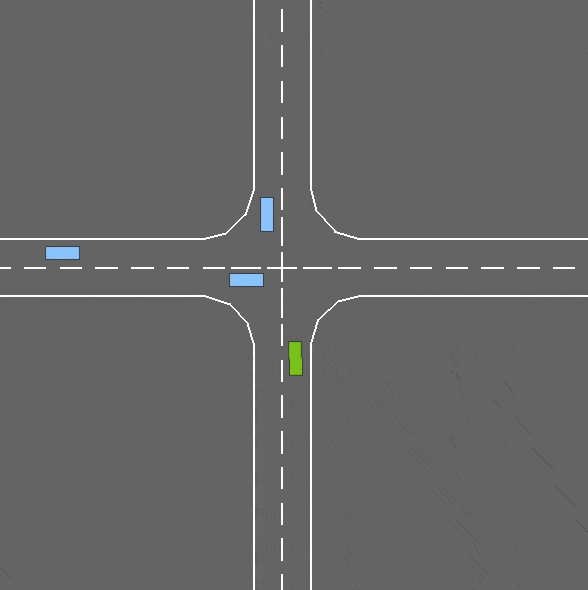
\includegraphics[width=8cm]{assets/highway}
    \caption{highway-env Simulator}
    \small
    Top view of the highway-env simulator, where the ego-vehicle (green) navigates an intersection with other vehicles (blue)\label{fig:figure9}
\end{figure}
To use highway-env, users can install it using pip and then import the environment in Python code. The agent can interact with the environment by taking actions, receiving observations, rewards, and additional information at each step.

Overall, highway-env offers a comprehensive set of environments for researchers and developers to study and develop autonomous driving algorithms and tactical decision-making strategies.

Highway-env may not be ideal for multi-agent RL research due to its primary focus on single-agent driving scenarios. The environment is specifically designed for studying the behavior of a single ego-vehicle navigating through various highway and road scenarios. While it provides a range of driving challenges for a lone agent, it lacks built-in support and mechanisms for handling multiple agents and their interactions.

In multi-agent RL research, environments need to accommodate complex interactions between multiple agents, where the actions of each agent can influence the behavior of others. Highway-env is not explicitly designed to handle such multi-agent dynamics, and modifying it to support multiple agents could be non-trivial and may not produce optimal results.

For comprehensive multi-agent RL research, specialized environments that explicitly cater to multi-agent scenarios, such as cooperative or competitive driving situations, are more appropriate. These environments should facilitate communication and coordination between agents, support joint learning, and provide tools for studying emergent behaviors arising from multi-agent interactions.

\subsection{MetaDrive}\label{subsec:metadrive}
\paragraph
MetaDrive~\cite{li2021metadrive} is a driving simulator designed for generalizable RL research\footnote{https://github.com/metadriverse/metadrive}. It supports generating diverse driving scenarios with various road maps and traffic settings, making it suitable for studying RL agents' generalization capabilities. The simulator is lightweight, easy to install, and can achieve up to 300 FPS on a standard PC. It provides realistic physics simulation and multiple sensory inputs, including Lidar, RGB images, top-down semantic maps, and first-person view images. Examples of different driving scenarios are provided, such as Single Agent Environment, Multi-Agent Environment, and Real Environment, along with instructions on how to run them. To build the RL environment, users can code in the Gymnasium format using the provided MetaDriveEnv class.
\begin{figure}[H]
    \centering
    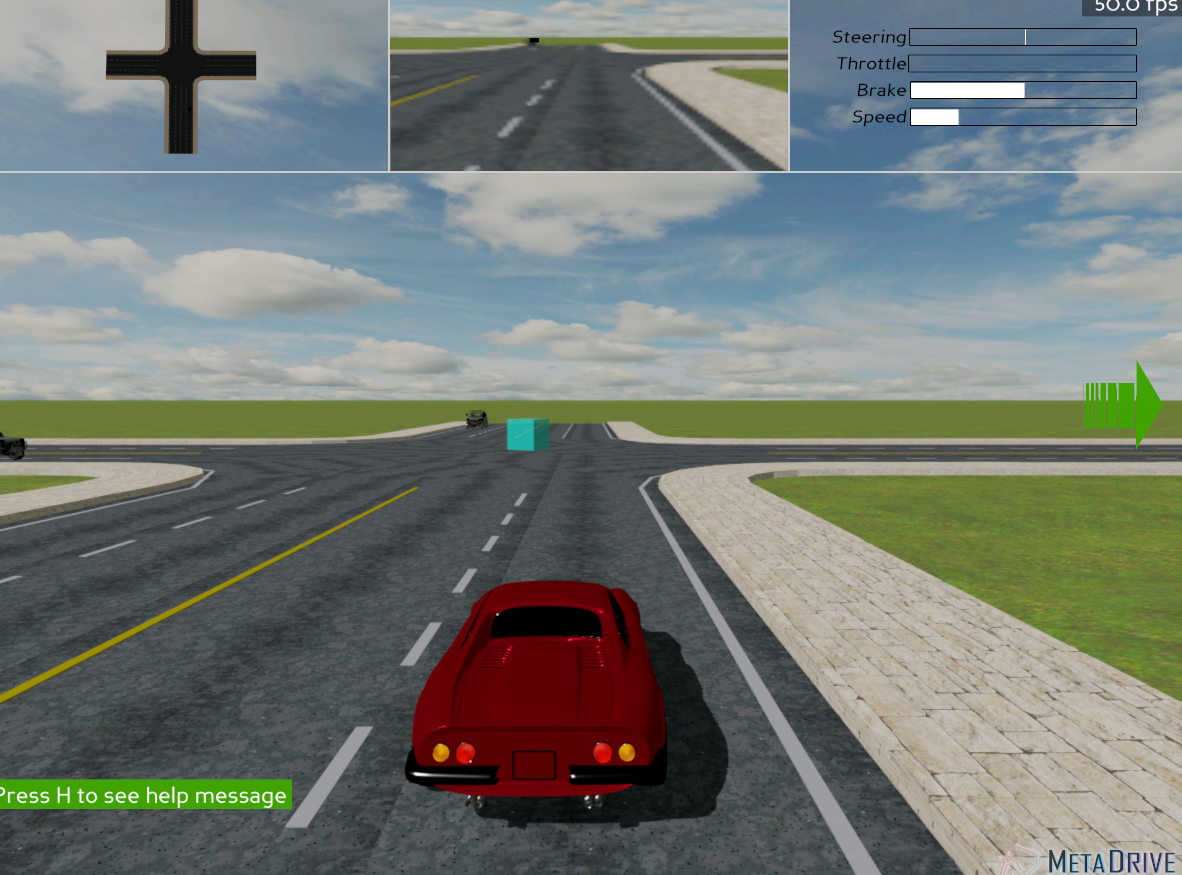
\includegraphics[width=10cm]{assets/meta-screen}
    \caption{MetaDrive Simulator}
    \small
    First person view of MetaDrive simulator showing mini-map, first person view, and top-down view\label{fig:metadrive-fig}
\end{figure}
MetaDrive stands out as an excellent choice for multi-agent RL research due to its provision of rich observations and robust multi-agent support. In the context of multi-agent RL, having access to diverse and comprehensive observations is crucial for agents to effectively learn and adapt in complex environments. MetaDrive addresses this need by offering multiple sensory inputs, including Lidar, RGB images, top-down semantic maps, and first-person view(FPV) images. These varied observation modalities enable agents to perceive the environment from different perspectives, promoting a more comprehensive understanding of the driving scenarios.

\begin{table}[H]
    \centering
    \caption{Comparison of 'gym-graph-traffic,' 'Highway-env,' and 'MetaDrive' for Multi-Agent RL Research}
    \label{tab:comparison}
    \begin{tabularx}{\textwidth}{@{}lXXX@{}}
        \toprule
        \multirow{2}{*}{\textbf{Feature}} & \textbf{gym-graph-traffic} & \textbf{Highway-env} & \textbf{MetaDrive}           \\
        \midrule
        Support for Multi-Agent           & No                         & No                   & Yes                           \\
        RL Research                       &                            &                      &                               \\
        \midrule
        Focus                             & Single-Agent               & Single-Agent         & Single and Multi Agent        \\
        & Traffic                    & Driving              & Driving                       \\
        \midrule
        Rich Observation                  & Limited                    & Limited              & Yes                           \\
        Modalities                        &                            &                      & (Lidar, RGB images, top-down  \\
        &                            &                      & semantic map, and FPV images) \\
        \midrule
        Multi-Agent                       & No                         & No                   & Limited                       \\
        Interactions                      &                            &                      & (Possible with modification)  \\
        \midrule
        Built for                         & Simple                     & Simple               & Realistic and                 \\
        Complex                           & Intersections              & Highways             & Diverse Driving               \\
        Scenarios                         &                            &                      & Scenarios                     \\
        \bottomrule
    \end{tabularx}
\end{table}
Furthermore, MetaDrive's multi-agent support is a key strength that sets it apart. In multi-agent environments, interactions and cooperation between agents play a significant role in determining their overall performance and behavior. MetaDrive facilitates the simulation of multiple agents simultaneously, allowing researchers to study cooperative, competitive, and mixed interactions between agents. This capability is invaluable for investigating complex real-world scenarios where multiple autonomous vehicles, pedestrians, and traffic participants interact dynamically.
By combining rich observations with multi-agent support, MetaDrive provides a versatile platform for exploring diverse driving scenarios, such as intersection negotiations, cooperative lane merging, and complex traffic situations. The ability to model and train agents in such realistic and interactive environments fosters the development of more robust and generalizable multi-agent RL algorithms, contributing significantly to the advancement of autonomous driving systems and intelligent transportation technologies. As a result, MetaDrive emerges as a superior option for researchers seeking a comprehensive and effective tool for multi-agent RL research in driving and traffic-related domains.





